\Chapter{Fejlesztői dokumentáció}
\label{Chap:dokumen}

\iffalse
Ebben a fejezetben kell a hallgatónak leírnia a saját eredményeit. Például ilyennek tekinthető a hallgató által elkészített program leírása, algoritmus leírása alkalmazási lehetőségek, eredmények. Lehet benne több alfejezet vagy al-alfejezet is. Ezek számozása és a tartalomjegyzékben  való megjelenítése rögzített. A fejezet címe megváltoztatható az eredmények szerint. Ez a fejezet és a \aref{Chap:tema} együtt összesen 25-60 oldal terjedelmű kell hogy legyen
\fi

Az Elméleti kifejtés során meghatározott célokat különböző gépi tanulási módszerekkel lehet megoldani amik eltérő eredménnyel, pontossággal fognak működni. A nehézségi osztályok meghatározására elsősorban a  \myaref{ssec:klaszterezes} pontban részletezett klaszterezési módszerek használhatóak

\Section{Adathalmaz előkészítés}
A fejlesztés legelső lépése az összegyűjtött adatok megfelelő struktúrára való átalakítása és megtisztítása, ezzel megkönnyítve a későbbi feldolgozást valamint növelve a gépi tanulási algoritmusok pontosságát

\SubSection{Adatstruktúra kialakítása}
Az adatgyűjtés elsődleges eszközeként a szakdolgozat keretein belül készített weboldal szolgált, amely minden információt egy JSON alapú adatbázisban tárolt le. Az adathalmaz előkészítésének a legelső lépése a JSON struktúráról való áttérés egy, a Python programozási nyelv által kezelt, könnyen használható adatstruktúrára. Erre a szakdolgozat során a Pandas \cite{python-pandas} nevű Python csomag által megvalósított DataFrame nevű struktúra fog szolgálni , amely segítségével az adatokat táblázathoz hasonló formában lehet tárolni. Egy DataFrame oszlopai egyedi, a fejlesztő által definiált oszlopnevekkel érhetőek el, soraira index használatával lehet hivatkozni. Az oszlopok egyenként különböző típusúak lehetnek és tartalmazhatnak NULL értékeket. A DataFrame egyik legnagyobb előnye az oszlopok nevesítése, amivel könnyen nyomon követhető hogy az aktuális értékek melyik feature-nek felelnek meg, mit reprezentálnak a valóságban

\begin{programreszlet}
A  parancs segítségével a JSON struktúra (jsonData) könnyen átalakítható DataFrame-é (dataset). A dataset oszlopai megfelelnek a \myaref{ssec:adatstruktura} pontban részletezett adatoknak.
\begin{python}
import pandas

jsonData = pandas.read_json("2019_02_08_10h.json", type='series')
cleanData = []
for u in userData:
  if userData[u]['connectedToStrava'] == True:
    for i in range(0,len(userData[user]['activities'])):
       userData[u]['activities'][i]['ageGroup'] = userData[u]['ageGroup']
       userData[u]['activities'][i]['sex'] = userData[u]['sex']
       userData[u]['activities'][i].pop('external_id', None)
       userData[u]['activities'][i].pop('map_id', None)
       userData[u]['activities'][i].pop('map_resource', None)
       userData[u]['activities'][i].pop('map_summary', None)
       cleanData.append(userData[u]['activities'][i]) 
  else:
    print('User does not have any activities')
dataset = pandas.DataFrame(cleanData)

\end{python}
\end{programreszlet}


A fenti parancs segítségével a JSON struktúra (jsonData) könnyen átalakítható DataFrame-é (dataset). A dataset oszlopai megfelelnek a \myaref{ssec:adatstruktura} pontban részletezett adatoknak.


\SubSection{Adattisztítás}
A megfelelő adatstruktúra kialakítása után a következő lépés az adatok megtisztítása. Ez a lépés azért szükséges mert a legfigyelmesebben gyűjtött adathalmaz is tartalmazhat rossz értékeket illetve előfordulhat hogy több helyen hiányzik a valódi érték. Ezeknek a hibáknak a megtalálása és kijavítása több fázisból áll.

\csvautotabular{adat/rawDataDescription.csv}


\subsubsection{NULL értékek}
Egy általános adatbázis esetén gyakran előfordul hogy egyes oszlopok NULL értékeket tartalmaznak - ebben az esetben például NULL jelöli ha egy útvonal nincs elérhető adat egy adott jellemzőről. Azonban a gépi tanulási algoritmusok számokat képesek feldolgozni így elengedhetetlen a NULL értékek kiküszöbölése valamilyen formában.

A NULL értékek kiküszöbölésére két elterjedt megoldás létezik:
\begin{itemize}
	\item \textbf{NULL értékek törlése:} az egyszerűbb megoldás a NULL értékeket tartalmazó sorok törlése, azonban ennek a módszernek nagy hátránya hogy sok NULL-t tartalmazó adathalmaz esetén jelentős mértékben megcsappan az adathalmaz mérete
	\item \textbf{NULL értékek feltöltése:} összetettebb, azonban sok esetben célravezetőbb megoldást jelent a NULL értékek helyettesítése valamilyen számított értékkel. Az új értékek számítása különböző módokon történhet, ez nagyban függ az adott jellemző jellegétől
\end{itemize}
Amennyiben egy oszlop nagy mértékben tartalmaz NULL értékeket érdemes megfontolni az elvetését vagy külön esetként kezelni mikor van tényleges érték

Az adat vizsgálata után az első szembetűnő gond a hiányzó értékek. Az alábbi jellemzők akkora mértékben hiányosak hogy a javításuk reménytelen feladat, így az adattisztítás elején törlésre kerültek.
\begin{itemize}
	\item average\_watts: 18.45\% hasznos értéket tartalmaz
	\item commute: 98.83\% hasznos értéket tartalmaz azonban ezekből csupán 23 True érték
	\item device\_watts : 19.56\%
	\item flagged : 19.56\%
	\item has\_heartrate : 19.56\%
	\item heartrate\_opt\_out: 
	\item kilojoules : 17.63\%
	\item max\_watts 5.54\%
	\item pr\_count : 19.56\%
	\item resource\_state : 19.56\%
	\item weighted\_average\_watts : 5.45\%
	\item sex : 100\% hasznos azonban elenyészően kevés női adatot tartalmaz az adathalmaz, ezért a torzítatlanság érdekében a szakdolgozat során csak a férfi útvonalak kerülnek felhasználásra - így ez az jellemző funkcióját veszti, konstans érték
	\item start\_latlng : 18.34\%
	\item end\_latlng : 18.34\%
\end{itemize}


\subsubsection{Kiugró értékek}
Gyakori jelenség hogy egy jellemző tartalmaz néhány magasan kiugró értéket, amelyek sokszor érvényesek azonban fakadhatnak mérési / rögzítési hibából is. Akár érvényes értékek, akár valamilyen hibából erednek érdemes kiküszöbölni őket mivel könnyen eltorzíthatják az eredményeket. 

A kiugró értékek megtalálása egy alapvető módszer került felhasználásra a szakdolgozat készítése során. A kiugró értékeket jellemzőként külön vizsgáljuk. $F$ jellemzőre $x \in F$ érték kiugrónak tekinthető amennyiben

\[  \frac{x - \overline{F}}{\sigma} > 2.5\]
teljesül, ahol $\overline{F}$ az $F$ jellemző átlaga, $\sigma$ pedig $F$ szórása.

Az alábbiakban a különböző jellemzők kiugró érték vizsgálatának jellemzése található.

\textbf{average\_speed (átlagsebesség):}

Ez a jellemző m/s-al adja meg az útvonal átlagsebességét. A fenti módszer 10 kiugró értéket talált amik 2182 m/s (7855.2 km/h) és 28290 ms/s (101844.0 km/h) közé esnek. Ekkora sebesség elérése nyilvánvalóan lehetetlen kerékpárral, eredetük az adatsorok megvizsgálása után leszűkíthető a mozgási idő (moving\_time) jellemző mérésének a hiányára / hibájára. Az átlagsebesség számítása ugyanis a távolság és a mozgási idő hányadosaként kerül kiszámításra és a vizsgált kiugró értékeknél a mozgási idő mindenhol 1 másodperc míg a távolság 10 km fölött van. Ezen adatok javítása nem tűnik megvalósíthatónak. Eldobásuk után az adathalmaz 10004 utat tartalmaz.

\textbf{distance (távolság):}

A distance jellemző méterben megadva tárolja az egy-egy útvonal során megtett távolságot. Kiugró érték vizsgálat során 313 értéket talált a módszer, amik között a legkisebb értéke 99915.1 méter azaz közel 100 km. Ezek az adatsorok azonban minden más szempontból helyes értékeket tartalmaznak és valójában a 100 km-s utak sem lehetetlenek. Ezek az értékek nem kerültek törlésre az adathalmazból azonban a későbbiek során érdemes lehet a hasonlóan hosszú utakat külön kezelni

\textbf{elev\_high (legmagasabb tengerszint feletti pont):}

Az elev\_high jellemző vizsgálata során 61 kiugró érték jelzett a módszer amelyek 976.6 méter és 12103.0 méter közé esnek. A 12103 méter egyértelműen lehetetlen, a többi érték pedig vele együtt elvetésre kerül. Ezen adatsorok eldobása után az adathalmaz 9943 útvonalat tartalmaz

\textbf{max\_speed (legnagyobb sebesség)}

A max\_speed az útvonal során mért maximális sebességet jelzi m/s mértékegységben. Vizsgálata során a használt módszer 218 kiugró értéket talált. Ezek az értékek két intervallumra oszthatóak fel. 0.0 m/s - 2.1 m/s és 22.1 m/s - 122.7 ms azaz 0.0 km/h - 7.56 km/h és 79.56 km/h - 441.72 km/s. Ezek olyan adatok amelyek kilógnak az adathalmazból, sok közülük lehetetlen / értelmezhetetlen. Ezen adatsorok eldobása után az adathalmaz 9725 útvonalat tartalmaz.

\textbf{moving\_time (mozgási idő)}

A moving\_time jellemző a tényleges mozgással töltött időt tárolja másodpercben megadva. A jellemző vizsgálata során 276 érték bizonyult kiugrónak amelyek közül a legkisebb értéke 16814 másodperc azaz nagyjából 4 óra és 40 perc. Ezek az értékek összefüggnek a távolság (distance) jellemző vizsgálata során talált kiugró értékekkel, így egyenlőre az adathalmaz része marad, a későbbiek során azonban külön lesz kezelve.


A kiugró értékek megtalálására használt módszeren felül definiálásra került néhány szabály amik segítségével ki lehet szűrni az egyéb helytelen adatokat. Ezek alapján elvetésre kerülnek azok az adatsorok ahol:
\begin{itemize}
	\item az átlagsebesség kisebb mint 2 m/s (7.2 km/h)
	\item a távolság kisebb mint 100 méter (néhány száz méter esetén előfordulhat hogy rövid sprinteket tettek meg a sportolók)
	\item a legmagasabb vagy legalacsonyabb tengerszint feletti magasság hiányzó adat
\end{itemize} 
Továbbá 2 helyen javításra került az összes eltelt idő (elapsed\_time) mivel kevesebb volt mint a mozgással tölött idő (moving\_time)


A fentebbi adatsorok eldobása után összességében 9603 útvonalat tartalmazó adathalmaz maradt.


\SubSection{Adatok áttekintése}
A további feldolgozás illetve a tényleges gépi tanulási algoritmusok felhasználása előtt érdemes kicsit mélyrehatóbban tanulmányozni az adathalmazt, felfedezni a mintákat és összefüggéseket. 

\begin{figure}[h!]
	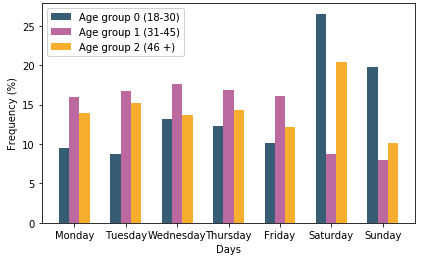
\includegraphics[width=\linewidth]{kepek/frequencyByAgeAndWeekdays.png}
	\caption{Activity frequency by days of week.}
	\label{fig:frequencyByWeekdays}
\end{figure}

Szöveg a fenti képről....

Blablabla

Még mindig.....




\begin{figure}[h!]
	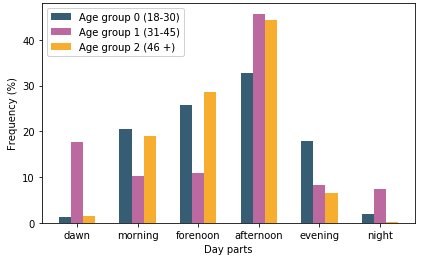
\includegraphics{kepek/frequencyByAgeAndDayparts.png}
	\caption{Activity frequency by dayparts.}
	\label{fig:frequencyByDayparts}
\end{figure}


Szöveg a fenti képről....

Blablabla

Még mindig.....


\begin{figure}[h!]
	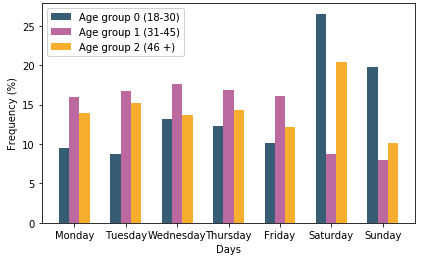
\includegraphics[width=\linewidth]{kepek/frequencyByAgeAndWeekdays.png}
	\caption{Activity frequency by days of week.}
	\label{fig:frequencyByWeekdays}
\end{figure}

Szöveg a fenti képről....

Blablabla

Még mindig.....




\begin{figure}[h!]
	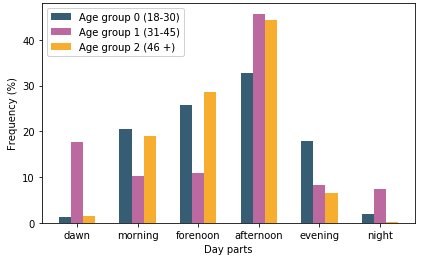
\includegraphics{kepek/frequencyByAgeAndDayparts.png}
	\caption{Activity frequency by dayparts.}
	\label{fig:frequencyByDayparts}
\end{figure}


Szöveg a fenti képről....

Blablabla

Még mindig.....





\SubSection{További adat feldolgozás}

\subsubsection{One-hot encoding}
A kiugró értékek kezelése és a adathalmaz összefüggéseinek vizsgálata után a következő lépés a one-hot encoding. Az eljárás lényege hogy egy kategória alapú jellemzőt több (a kategóriák számának megfelelő) oszlopra bont szét, ahol az egyes oszlopokban, jellemzőkben 1-es szerepel amennyiben az adatsor abba az adott kategóriába sorolható, 0 egyébként. Ennek az előnye hogy kiküszöböli a kategóriák sorszámmal történő jelzésének távolságát. Például egy korcsoportot tároló jellemző esetén nem biztos hogy helyes feltételezni hogy a 0. és a 2. kategória (csoport) között 2 távolság van. A one hot encoding természetesen folytonos változók esetén nem értelmezhető és kategoriális jellemzőkre sem mindig érdemes alkalmazni.

A szakdolgozathoz használt adathalmaz esetén 3+1 jellemző kerül one-hot encode-olásra: age\_group (korcsoport), workout\_tpye, start\_date\_local és a training.

\textbf{age\_group:} a sportoló korcsoportját jelzi, értékei egy három elemű halmazból kerülhetnek ki: \{0,1,2\} ahol 0 a [18,30], 1 a [31,45] 2 pedig a [46,$+\infty$] korcsoportokba való tartozást jelenti. One-hot encoding során az eredeti jellemzőből 3 oszlop készül, végül az eredeti törlésre kerül az adathalmazból.
\begin{programreszlet}
Python parancsok részletezése
\begin{python}
ageOneHot = pandas.get_dummies(rawData['age_group'], prefix='age')
rawData.drop(columns=['age_group'], inplace=True)
rawData = rawData.join(ageOneHot)
\end{python}
\end{programreszlet}
A kódban megadott prefix paraméter segítségével az új jellemzők nevei: age\_0.0, age\_1.0, age\_2.0


\textbf{workout\_tpye:} 

\begin{programreszlet}
\begin{python}
workoutTypeOneHot = pandas.get_dummies(rawData['workout_type'], prefix='workout_type')
rawData.drop(columns='workout_type', inplace=True)
rawData = rawData.join(workoutTypeOneHot)
\end{python}
\end{programreszlet}


\textbf{start\_date\_local:} a jellemző az aktivitás kezdeti idejét tárolja, a sportoló saját időzónája szerint, ÉÉÉÉ-MM-DD HH:MM:SS formátumban. Dátum mezők azonban nem értelmezhetőek gépi tanulási algoritmusokkal így a jellemző átalakítása szükségszerű volt. A dátumból alapvetően 2 féle új jellemző kerül kinyerésre, majd ezek külön kerülnek one-hot encode-olásra

\begin{programreszlet}
Az aktivitás kezdetének dátumából kinyerhető hogy a hét melyik napján történt az aktivitás. Ennek az információnak a kinyerését és one-hot encode-olását az alábbi kód végzi
\begin{python}
rawData['day_of_week'] = rawData['start_date_local'].dt.day_name()
weekDayOneHot = pandas.get_dummies(rawData['day_of_week'], 
				   prefix='weekday')
rawData.drop(columns=['day_of_week'], inplace=True)
rawData = rawData.join(weekDayOneHot)
\end{python}		
\end{programreszlet}

\begin{programreszlet}
Az aktivitás kezdetének időpontjából kinyerhető hogy melyik napszakban kezdődött az aktivitás. Ennek az információnak a kinyerését és one-hot encode-olását az alábbi kód végzi
\begin{python}
rawData['daypart'] = rawData['start_date_local'].apply(lambda row: 
						 timeToPartOfDay(row))
dayPartOneHot = pandas.get_dummies(rawData['daypart'], prefix='daypart')
rawData.drop(columns=['daypart'], inplace=True)
rawData = rawData.join(dayPartOneHot)
\end{python}	

Ahol a timeToPartOfDay függvény a start\_date\_local jellemző minden adattagjára külön hívódik meg. Ez a függvény szubjektíven oszt fel egy napot hat napszakra \myaref{fig:daypartsClock} ábra szerint

\begin{figure}[!h]
\centering
\begin{tikzpicture}[line cap=rect,line width=3pt]
\filldraw[fill=chart5, draw=chart5, line width=1pt] (0,0)-- +(45:2) arc (45:0:2); %hajnal
\filldraw[fill=chart0, draw=chart0, line width=1pt] (0,0)-- +(120:2) arc (120:45:2); %éjszaka
\filldraw[fill=chart1, draw=chart1, line width=1pt] (0,0)-- +(180:2) arc (180:120:2); %este
\filldraw[fill=chart2, draw=chart2, line width=1pt] (0,0)-- +(270:2) arc (270:180:2); %délután
\filldraw[fill=chart3, draw=chart3, line width=1pt] (0,0)-- +(315:2) arc (315:270:2); %délelőtt
\filldraw[fill=chart4, draw=chart4, line width=1pt] (0,0)-- +(360:2) arc (360:315:2); %reggel

\node[font=\small] at (90:2.36cm) {\textsf{Éjszaka}};
\node[font=\small] at (20:2.7cm) {\textsf{Hajnal}};
\node[font=\small] at (340:2.7cm) {\textsf{Reggel}};
\node[font=\small] at (305:2.6cm) {\textsf{Délelőtt}};
\node[font=\small] at (215:2.7cm) {\textsf{Délután}};
\node[font=\small] at (155:2.6cm) {\textsf{Este}};

\draw (0,0) circle [radius=2cm];

\foreach \angle [count=\xi] in {75,60,...,-270}
{
	\draw[line width=1pt] (\angle:1.8cm) -- (\angle:2cm);
	%\node[font=\small] at (\angle:1.36cm) {\textsf{\xi}};
}
\foreach \angle [count=\xi] in {0,45,90,135,180,225,270,315}
{
	\draw[line width=2pt] (\angle:1.6cm) -- (\angle:2cm);
}
\draw (0,0) -- (120:0.8cm);
\draw (0,0) -- (90:1cm);
\node[font=\small] at (0:1.36cm) {\textsf{6}};
\node[font=\small] at (45:1.36cm) {\textsf{3}};
\node[font=\small] at (90:1.36cm) {\textsf{0}};
\node[font=\small] at (135:1.30cm) {\textsf{21}};
\node[font=\small] at (180:1.36cm) {\textsf{18}};
\node[font=\small] at (225:1.36cm) {\textsf{15}};
\node[font=\small] at (270:1.36cm) {\textsf{12}};
\node[font=\small] at (315:1.36cm) {\textsf{9}};


%\filldraw[line color=gray!40 ] -- +(45:2) arc (45:-45:2);
\end{tikzpicture}
	\caption{Napszakok kialakítása.}
\label{fig:daypartsClock}
\end{figure}
\end{programreszlet}


\textbf{trainer: } a trainer jellemző Igaz / Hamis értékekkel jelzi hogy egy adott aktivitás traineren, azaz gépen történt e, nem pedig tényleges kerékpáron. Ennek a jellemzőnek az átalakítása nem igazi one-hot encoding, inkább csak az Igaz / Hamis értékek átmappelése 1 / 0 értékekre.  


Az adattisztítás összes lépése után az adathalmaz szerkezete lényegesen megváltozik, új jellemzőket tartalmaz (one-hot encoding) valamint az eddigi jellemzők sok esetben más intervallumokba esnek (kiugró értékek kezelése).

Jellemzők:
\begin{itemize}
	\item average\_speed
	\item distance
	\item elapsed\_time
	\item elev\_high
	\item elev\_low
	
	\item hashed\_id 
	\item max\_speed
	\item moving\_time
	\item total\_elevation\_gain
	\item age\_0.0 
	\item age\_1.0
	\item age\_2.0
	\item trainer\_onehot
	\item workout\_type\_0.0
	\item workout\_type\_4.0 
	\item workout\_type\_10.0 
	\item workout\_type\_11.0
	\item workout\_type\_12.0
	\item weekday\_Friday 
	\item weekday\_Monday
	\item weekday\_Saturday 
	\item weekday\_Sunday 
	\item weekday\_Thursday
	\item weekday\_Tuesday', 
	\item weekday\_Wednesday', 
	\item daypart\_afternoon',
	\item daypart\_dawn', 
	\item daypart\_evening', 
	\item daypart\_forenoon',
	\item daypart\_morning', 
	\item daypart\_night
\end{itemize}


az adathalmaz mentésre kerül a későbbi felhasználás megkönnyítésének céljából. A tisztított adatot a \textit{data\_advanced\_date.csv} fájl tartalmazza


% ADATTISZTITAS VEGE


% ML KEZDETE

\Section{Gépi tanulás}


\SubSection{Mozgási és eltelt idő számítása}

Az adathalmaz egy aktivitásra tekintve két különböző időtartamot különböztet meg: a mozgással töltött (moving\_time) és az összesen eltelt (elapsed\_time) időt, mindkettőt másodpercben mérve. A szakdolgozat során ennek a két időtartamnak a várható értékének a meghatározása az egyik cél gépi tanulási algoritmusokkal valamint ezen algoritmusoknak az összehasonlítása. Ennek a feladatnak a megoldásához a  \myref{subsec:regression} alfejezetben kifejtett regressziók adnak alapot.

A kétféle időtartam alapvetően külön kezelve, egyenként kerül becslésre, erre kivételt fog jelenteni a \TODO href pontban részletezett MLPRegressor.

\subsubsection{Mozgási idő (moving\_time)}
A tisztított adathalmaz beolvasása után szükséges kialakítani az $X$ és $y$ halmazokat amelyek a \TODO adatokat tartalmazzák. Az $y$ fogja tartalmazni a moving\_time jellemzőt míg $X$ minden mást ami alapján $y$ megbecsülhető. 

A regressziók során nagyon fontos az adathalmaz skálázása, egy intervallumra hozása. Ennek fontossága akkor mutatkozik meg igazán mikor a különböző jellemzők nagyon eltérő intervallumokba esnek, például az average\_speed 2.03 és 12.478 értékek között mozog míg a distance 161 és 436806 között. Ezért a gépi tanulás során gyakran alkalmazott eljárás az adathalmaz normalizálása vagy standardizálása amely az összes jellemzőt egy szűk intervallumra vetíti le. A standardizálás elvégzésére a szakdolgozat során a scikit-learn csomag által biztosított StandardScaler függvény szolgált

\begin{programreszlet}   
szöveg

\begin{python}
from sklearn.preprocessing import StandardScaler
X = dataset.copy()

names = X.columns
scaler = StandardScaler()

scaledData = scaler.fit_transform(X)
scaledData = pandas.DataFrame(scaledData, columns=names)
\end{python}
\end{programreszlet}

\begin{programreszlet} A túltanulás elkerülése érdekében a tanító és cél adathalmazokat szét kell osztani tanító és tesztelő részekre. A regressziós modellek csak a tanító (train) adatokon fognak tanulni, ellenőrzésre, pontosság meghatározására pedig a teszt (test) adatok szolgálnak.  \TODO
\begin{python}
from sklearn.model_selection import train_test_split
	
scaledY = scaledData['moving_time']
scaledData.drop(columns=['moving_time','elapsed_time'], inplace=True)

trainX, testX, trainy, testy = train_test_split(scaledData, scaledY, 
						random_state=42)
\end{python}

\end{programreszlet}

\textbf{Ridge regresszió:} ez az algoritmus 2 paraméterrel finomhangolható: $\alpha$ és solver. \TODO kifejtés. A moving\_time esetén a standardizált adathalmazra a legoptimálisabb (legnagyobb pontosságot eredményező paraméterek) a $\alpha = 0.003$ solver : saga. Ezeknek az alkalmazása esetén, a modellt a trainX és trainy adathalmazokon tanítva a pontosság 96.251\% (a teszt adatokon). A modell nem tanul túl, mivel a teszt adatokon (amiket a modell tanulás során nem ismer) nagy pontosság jellemzi a regressziót.

\textbf{Lasso regresszió:} 
$\alpha = 0.0001$, pontosság: 96.246\%

%\Section{Programkód}
